% !TEX TS-program = lualatex
% !TEX encoding = UTF-8 Unicode

\documentclass[12pt, letterpaper]{article}

%%BIBLIOGRAPHY- This uses biber/biblatex to generate bibliographies according to the
%%Unified Style Sheet for Linguistics
\usepackage[main=american, german]{babel}% Recommended
\usepackage{csquotes}% Recommended
\usepackage[backend=biber,
        style=unified,
        maxcitenames=3,
        maxbibnames=99,
        natbib,
        url=false]{biblatex}
\addbibresource{homework.bib}
\setcounter{biburlnumpenalty}{100}  % allow URL breaks at numbers
% \setcounter{biburlucpenalty}{100}   % allow URL breaks at uppercase letters
% \setcounter{biburllcpenalty}{100}   % allow URL breaks at lowercase letters

%%TYPOLOGY
\usepackage[svgnames]{xcolor} % Specify colors by their 'svgnames', for a full list of all colors available see here: http://www.latextemplates.com/svgnames-colors
\usepackage[hmargin=1in,vmargin=1in]{geometry}  %Margins          
\usepackage{graphicx}	%Inserting graphics, pictures, images 		
\usepackage{stackengine} %Package to allow text above or below other text, Also helpful for HG weights 
\usepackage{fontspec} %Selection of fonts must be ran in XeLaTeX or LuaLateX
\usepackage{amssymb} %Math symbols
\usepackage{amsmath} % Mathematical enhancements for LaTeX
\usepackage{setspace} %Linespacing
\usepackage{multicol} %Multicolumn text
\usepackage{enumitem} %Allows for continuous numbering of lists over examples, etc.
\usepackage{multirow} %Useful for combining cells in tablesbrew 
\usepackage{hanging}
\usepackage{fancyhdr} %Allows for the 
\pagestyle{fancy}
\fancyhead[L]{\textit{LING 450/550: Homework 1}} 
\fancyfoot[L]{[Updated: \textit{\today}]}
\fancyfoot[C]{\thepage} 
\renewcommand{\headrulewidth}{0.4pt}
\setlength{\headheight}{14.5pt} % ...at least 14.49998pt
% \usepackage{fourier} % This allows for the use of certain wingdings like bombs, frowns, etc.
% \usepackage{fourier-orns} %More useful symbols like bombs and jolly-roger, mostly for OT
\usepackage[colorlinks,allcolors={black},urlcolor={blue}]{hyperref} %allows for hyperlinks and pdf bookmarks
% \usepackage{url} %allows for urls
% \def\UrlBreaks{\do\/\do-} %allows for urls to be broken up
\usepackage[normalem]{ulem} %strike out text. Handy for syntax
\usepackage{tcolorbox}
\usepackage{datetime2}
\usepackage{longtable}
\usepackage{booktabs}

%%FONTS
\setmainfont{Libertinus Serif}
\setsansfont{Libertinus Sans}
\setmonofont[Scale=MatchLowercase]{Libertinus Mono}

%%PACKAGES FOR LINGUISTICS
\usepackage[noipa]{OTtablx} % Use this one generating tableaux without using TIPA
\usepackage{langsci-gb4e} % Language Science Press' modification of gb4e
\usepackage{tikz} % Drawing Hasse diagrams
\usepackage{leipzig} %	Offers support for Leipzig Glossing Rules

%%LEIPZIG GLOSSING FOR ZAPOTEC
\newleipzig{el}{el}{elder} % Elder pronouns
\newleipzig{hu}{hu}{human} % Human pronouns
\newleipzig{an}{an}{animate} % Animate pronouns
\newleipzig{in}{in}{inanimate} % Inanimate pronouns
\newleipzig{pot}{pot}{potential} % Potential Aspect
\newleipzig{cont}{cont}{continuative} % Continuative Aspect
\newleipzig{stat}{stat}{stative} % Stative Aspect
\newleipzig{and}{and}{andative} % Andative Aspect
\newleipzig{ven}{ven}{venative} % Venative Aspect
% \newleipzig{res}{res}{restitutive} % Restitutive Aspect
\newleipzig{rep}{rep}{repetitive} % Repetitive Aspect

%%TITLE INFORMATION
% \title{TITLE}
% \author{Mykel Loren Brinkerhoff}
% \date{\today}

%%MACROS
\newcommand{\sub}[1]{\textsubscript{#1}}
\newcommand{\supr}[1]{\textsuperscript{#1}}

\makeatletter
\renewcommand{\paragraph}{%
  \@startsection{paragraph}{4}%
  {\z@}{0ex \@plus 1ex \@minus .2ex}{-1em}%
  {\normalfont\normalsize\bfseries}%
}
\makeatother
\parindent=10pt


\begin{document}

%%If using linguex, need the following commands to get correct LSA style spacing
%% these have to be after  \begin{document}
    % \setlength{\Extopsep}{6pt}
    % \setlength{\Exlabelsep}{9pt}		%effect of 0.4in indent from left text edge
%%

%% Line spacing setting. Comment out the line spacing you do not need. Comment out all if you want single spacing.
%	\doublespacing
%	\onehalfspacing

\begin{center}
    {\Large \textbf{LING 450/550: Homework 2}}\\
    {\large Due: Tuesday, October 7, 2025 at 8:30am}
\end{center}
%\maketitle
%\maketitleinst
\thispagestyle{fancy}

% \tableofcontents

%------------------------------------
%\section{} \label{}
%------------------------------------

\textbf{Please read all instructions carefully before starting the assignment.} The instructions include important information about all homeworks this quarter. If you have any questions, please ask them in class or via email.

\begin{tcolorbox}[colback=LightGray!10!white,colframe=LightGray!75!black,title=Instructions]
    \begin{itemize}
        \item Please submit your homework as a PDF file on Canvas by the deadline.
        \item You may work with other students in the class, but you must write up your solutions independently and in your own words. Please list any collaborators at the end of your assignment.
        \item You may use any resources you like, but please cite them appropriately using the \href{https://apastyle.apa.org/}{\textit{APA citation style}} or the \href{https://langsci-press.org/unifiedstylesheet}{Unified Style Sheet for Linguistics}. If you use online resources, please make sure they are reputable and reliable.
        \item Please make sure your solutions are clear and well-organized. Use headings, bullet points, and diagrams where appropriate to help illustrate your points.
        \item If you have any questions or need clarification on any part of the assignment, please don't hesitate to reach out to me or the TA via email or during office hours.
        \item AI tools (e.g., ChatGPT, Grammarly, Copilot, etc.) may be used to help with grammar, spelling, and formatting. However, you must ensure that all content is your own work and that you understand everything you submit. Please indicate in a footnote/endnote if you used any AI tools and for what purpose.
    \end{itemize}
\end{tcolorbox}

%------------------------------------
\section*{Part 1: Describing articulation} \label{sec:describingarticulation}
%------------------------------------

Please answer the following questions about articulatory phonetics. Your responses should be about 1-2 paragraphs for each question. 

\begin{enumerate}
    \item Describe how the vocal folds operate, with special attention to how \textit{voicing}, or vocal fold vibration works, including how we change the pitches of our voices
    \item Describe the velum’s function in speech. Your answer should include terms such as \textit{oral airflow}, \textit{nasal airflow}, as well as \textit{place of articulation}.
\end{enumerate}

%------------------------------------
\section*{Part 2: Labeling articulators} \label{sec:labelingarticulators}
%------------------------------------

Below is a midsaggital view of the vocal tract from \citet{forinashSoundInteractiveEBook2025}. Your task is to provide the appropriate names for each of the numbered parts in the midsaggital view. 
\begin{figure}[!h]
    \centering
    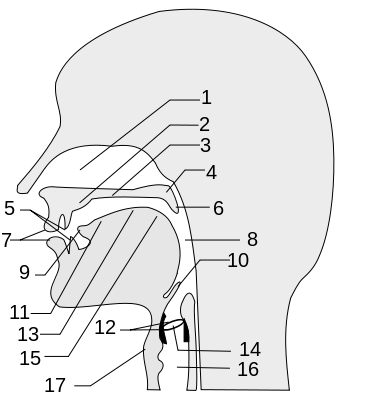
\includegraphics[width = .75\linewidth]{figs/VocalTract_Labeling.png}
\end{figure}

\begin{multicols}{2}
    \begin{enumerate}
        \setlength{\itemsep}{1em}
        \item \rule{5cm}{0.4pt}
        \item \rule{5cm}{0.4pt}
        \item \rule{5cm}{0.4pt}
        \item \rule{5cm}{0.4pt}
        \item \rule{5cm}{0.4pt}
        \item \rule{5cm}{0.4pt}
        \item \rule{5cm}{0.4pt}
        \item \rule{5cm}{0.4pt}
        \columnbreak
        \item \rule{5cm}{0.4pt}
        \item \rule{5cm}{0.4pt}
        \item \rule{5cm}{0.4pt}
        \item \rule{5cm}{0.4pt}
        \item \rule{5cm}{0.4pt}
        \item \rule{5cm}{0.4pt}
        \item \rule{5cm}{0.4pt}
        \item \rule{5cm}{0.4pt}
        \item \rule{5cm}{0.4pt}
    \end{enumerate}
\end{multicols}

%------------------------------------
\section*{Understanding the articulations}
%------------------------------------

On the following page, there are three partially complete vocal tract diagrams. For each diagram, you must complete the diagram for the consonantal sound that begins each corresponding word. Each diagram gets progressively harder. 

\begin{enumerate}
    \setlength{\itemsep}{2em}
    \item \textit{talk} \\
        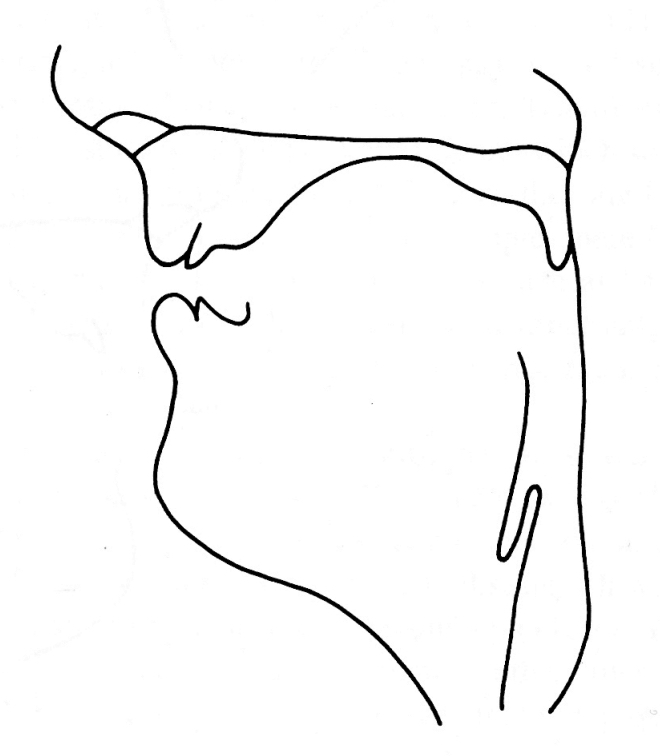
\includegraphics[width = .5\linewidth]{figs/MIdsaggital_t.jpg}
    \item \textit{chase} \\
        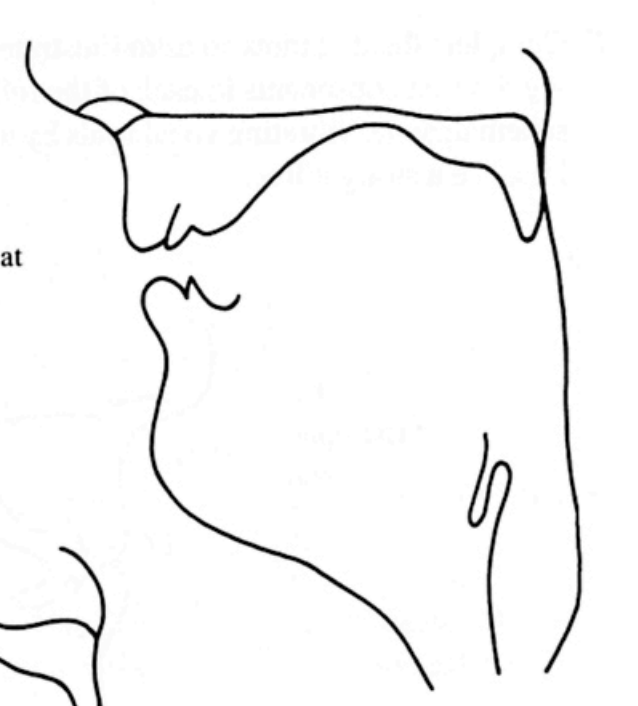
\includegraphics[width = .5\linewidth]{figs/Midsaggital_tS.png}
    \item \textit{knight}\\
        
\includegraphics[width = .5\linewidth]{figs/Midsaggital_n.png}
\end{enumerate}

%------------------------------------
%BIBLIOGRAPHY
%------------------------------------

%\singlespacing
%\nocite{*}
\printbibliography[heading=bibintoc]

\end{document}